\documentclass[12pt,fleqn,a4paper,]{LegrandOrangeBook}
\addbibresource{sample.bib} % Bibliography file
\definecolor{ocre}{RGB}{243, 102, 25} 
\chapterimage{orange1.jpg} 
\chapterspaceabove{6.5cm}
\chapterspacebelow{6.75cm} 
%\begin{theorem}[Name of the theorem]
%\begin{exercise}
%\begin{example}[Example name]
%\begin{definition}[Definition name]
%\begin{corollary}[Corollary name]
%\begin{remark}
%\begin{proposition}[Proposition name]
%\begin{problem}
%\begin{vocabulary}[Word]
%\begin{notation}
%----------------------------------------------------------------------------------------
\begin{document}
%----------------------------------------------------------------------------------------
%----------------------------------------------------------------------------------------
%Lineas
%----------------------------------------------------------------------------------------
\section{Leyes de maxwell}\index{Leyes de maxwell}
Se presentan las ecuaciones de Maxwell en la tabla \ref{tab:maxwell}.
\begin{table}[]
\begin{tabular}{|l|m{0.3\linewidth}|l|}
\hline
\rowcolor[HTML]{0066cc} 
Forma diferencial                                  & Forma integral                                                                 & Comentario                     \\ \hline
$\nabla\cdot \textbf{D}=\rho_v$                             & \begin{displaymath}
\oint_S\textbf{D}\cdot d\textbf{S}=\int_v\rho_vdv                                 \end{displaymath} & Ley de Gauss               \\ \hline
$\nabla\cdot \textbf{B}=0$                                  & \begin{displaymath}
\oint_S\textbf{B}\cdot d\textbf{S}=0
\end{displaymath}                                                           & No existencia de monopolos \\ \hline
$\nabla\times \textbf{E}=-\frac{\partial \textbf{B}}{\partial t}$    & \begin{displaymath}
\oint_L\textbf{E}\cdot dl=-\frac{\partial}{\partial t}\int_S\textbf{B}\cdot dS
\end{displaymath}                  & Ley de Faraday             \\ \hline
$\nabla\times \textbf{H}=\textbf{J} + \frac{\partial \textbf{D}}{\partial t}$ & \begin{displaymath}
\oint_L\textbf{H}\cdot dl=\int_S\left(\textbf{J} + \frac{\partial \textbf{D}}{\partial t}\right)\cdot d\textbf{S}
\end{displaymath} & Ley de circuitos de Ampere \\ \hline
\end{tabular}
\caption{Leyes de Maxwell}
\label{tab:maxwell}
\end{table}
Donde es necesario recordar el operador DEL (\ref{subsec:DEL})
\begin{itemize}
\item El gradiente de un escalar V: $\nabla$V
\item La divergencia de un vector A: $\nabla\cdot$A
\item La rotacional de un vector A: $\nabla\times$A
\item El Laplaciano de un escalar V: $\nabla^2$V
\end{itemize}
Además se tienen ecuaciones auxiliares:
\begin{subequations}
\begin{align}
\intertext{Relación entre la Densidad de Campo Eléctrico y la Intensidad de Campo Eléctrico.}
\textbf{D}&= \epsilon \textbf{E}\\
\intertext{Relación entre la Densidad de Campo Magnético y la Intensidad de Campo Magnético.}
\textbf{B}&=u\textbf{H}\\
\intertext{Densidad de Corriente de conducción.}
\textbf{J}&=\sigma\textbf{E}\\
\intertext{Densidad de Corriente de convección en función de la densidad de carga volumétrica.}
\textbf{J}&=\rho_v\textbf{v}
\end{align}
\end{subequations}
Hay ligeras modificaciones si son para conductores malos (aislantes):
\begin{subequations}
\begin{align}
\textbf{D}&= \epsilon \textbf{E} + P\\
\textbf{B}&=u(\textbf{H} + M)
\end{align}
\end{subequations}
Donde P es el campo de polarización y M es el campo de magnetización, cuando el dieléctrico es lineal se tiene:
\begin{align*}
&P=\chi_e\epsilon_0\textbf{E} &M=\chi_m\textbf{H}
\end{align*}
\begin{figure}[H]
\centering
\subfloat[Ecuación de onda para campos eléctricos.]{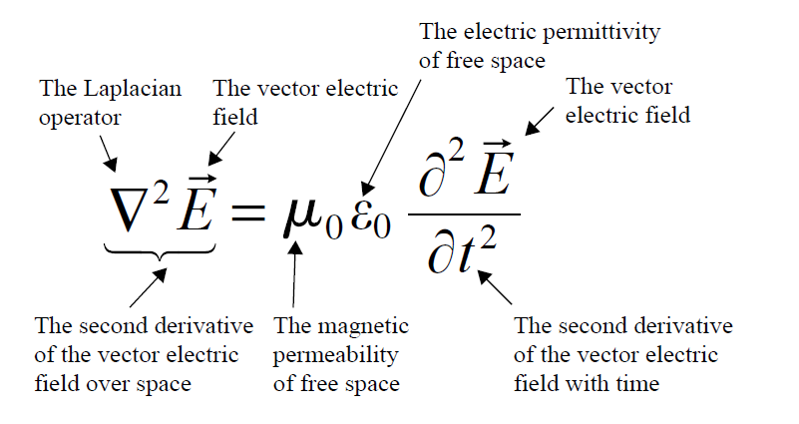
\includegraphics[width=0.8\linewidth]{LT/LT1.png}}\\
\subfloat[Ecuación de onda para campos magnéticos.]{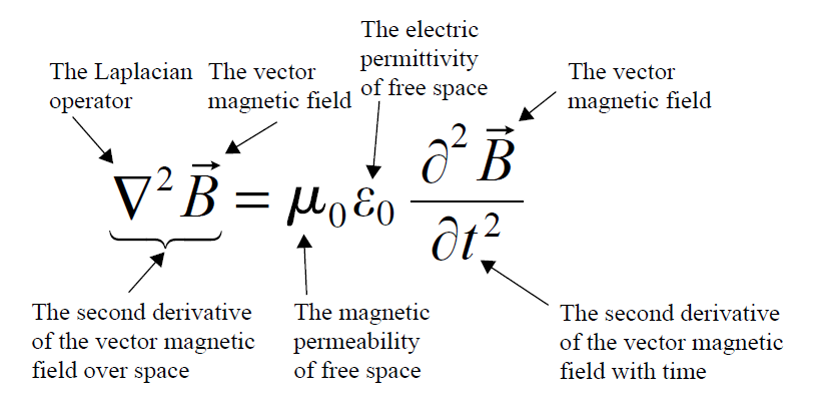
\includegraphics[width=0.8\linewidth]{LT/LT2.png}}
\caption{Ecuaciones de onda}
\end{figure}
%\section{Modelo electromagnético y las leyes de Maxwell}
%----------------------------------------------------------------------------------------
%Internetworking
%----------------------------------------------------------------------------------------
\begin{remark}
No confundir enrutamiento con direccionamiento. El primero se trata de saltar entre redes, por ejemplo mandar datos desde la LAN propia de un empresa hacia la LAN propia de otra empresa, los datos salen de nuestra red y viajan; mientras que el direccionamiento se trata dentro de la misma red, mandar a imprimir un archivo en una impresora LAN.
\end{remark}
Vale la pena recordar el contexto en el que estamos para trabajar la cada de red, esta se puede ver en la figura \ref{fig:entorno red}, el host 1 es una computadora conectada directamente al ISP (Proveedor de servicio de internet) representado por la región ploma, mientras que el host tiene un conexión que pasa a través de F, pudiendo ser una oficina con un router LAN.
\begin{figure}[]
\centering
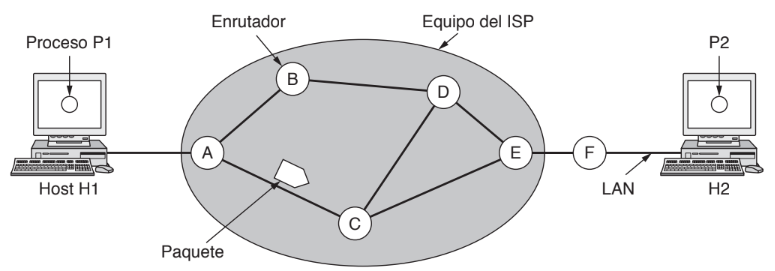
\includegraphics[width=0.7\linewidth]{IN1/IN57.png}
\caption{Entorno de los protocolos de la capa de red}
\label{fig:entorno red}
\end{figure}
Existen diferentes formas que un datagrama llegue de un punto a otro, estas puedes ser enviadas de diferentes maneras a través de la \textbf{red de datagramas} que solo es aplicada para las \textbf{conexiones no orientadas a la conexión} pues son enrutados de manera independiente. En la figura \ref{fig:enru datagrama} podemos ver que un flujo de datos ha sido fragmentado en 4 datagramas, además nos presentan las tablas de enrutamiento\footnote{Solo sirven a manera de ejemplo, no siempre son esos valores} que indican como van a viajar los datagramas, si vemos la tabla \textit{A} (al principio), notamos que la primera columna es el destino y la segunda la línea. La primera fila se ignora pues estamos ya en \textit{A}, la segunda fila será leída: \emph{Para enviar el datagrama a \textbf{\textit{B}}, usamos la línea hacia \textbf{\textit{B}}}. Esta misma sintaxis será usada par los demás cuadros, estos cuadros dependen de cada sistema y no son fijos, habrá caminos restringidos por alguna razón, por ejemplo en la tabla de \textit{C} notamos que para llegar a \textit{D}, no lo podemos hacer directo, sino que tenemos que pasar por \textit{E}. Los datagramas 1, 2 y 3 han sido enrutados por el mismo camino pero 4 ha sido enrutado por otro camino, esto es porque la tabla de \textit{A} ha sido cambiada por la de (más tarde), tal vez hubo tráfico por lo que se enruto por otro camino, para esto se usan \textbf{algoritmos de enrutamiento}.
\begin{figure}[H]
\centering
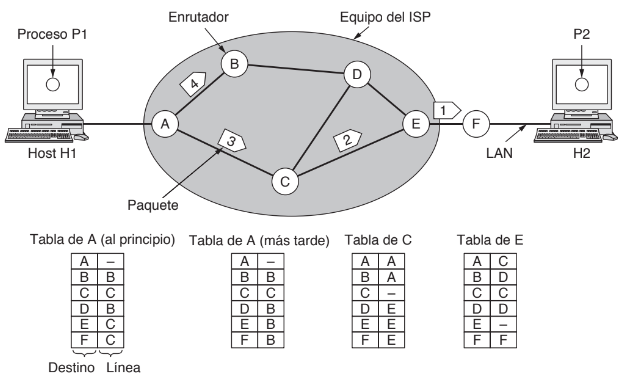
\includegraphics[width=0.8\linewidth]{IN1/IN58.png}
\caption{Enrutamiento dentro de una red de datagramas.}
\label{fig:enru datagrama}
\end{figure}
Mientras que para lo \textbf{servicios orientados a la conexión}, los caminos ya están definidos como se ve en al figura \ref{fig:circ virt}, estos caminos son llamados \textbf{circuitos virtuales} y la red es llamada \textbf{red de circuitos virtuales}. En cada enrutador ya se tiene configurada la ruta, todo tráfico fluye por esa conexión y cuando se libera, también se termina el circuito virtual. Aquí cada paquete lleva un identificador que indica a cuál circuito pertenece.
\begin{figure}[H]
\centering
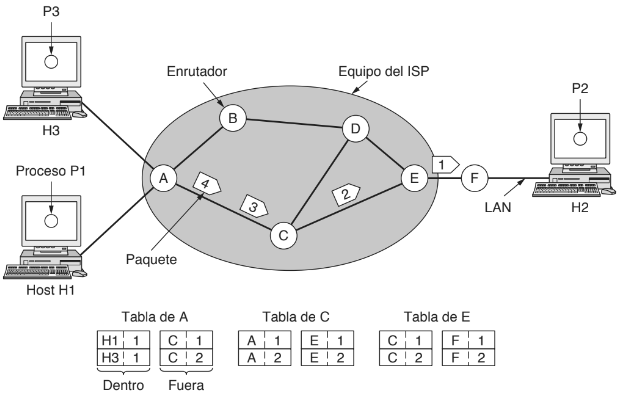
\includegraphics[width=0.8\linewidth]{IN1/IN59.png}
\caption{Enrutamiento dentro de una red de circuitos virtuales.}
\label{fig:circ virt}
\end{figure}
En la figura \ref{fig:circ virt}, la conexión entre \textit{H1} y \textit{H2} se ve plasmada en las primeras filas de cada tabla: tabla \textit{A}: si H1 con la etiqueta 1 llega a \textit{A}, está será enviada a \textit{C} con la etiqueta 1; en tabla \textit{C}, si llega de \textit{A} con la etiqueta 1, será enviada a \textit{E} con etiqueta 1 y así sucesivamente, sin embargo para H3 hay un error, pues también quiere comunicarse con H2, al llegar a \textit{A}, este si sabe cuales paquetes viene de H1 y cuales de H2, por los que lo etiqueta diferentes, pero esta información no la saben los demás pues solo se encargan de enviar y no les cambian las etiquetas. Por eso es importante asignar y reemplazar un identificador de conexión en los paquetes de salida.\\\textbf{MPLS} (conmutación mediante etiquetas) es un servicio orientado a la conexión. 
\begin{table}[H]
\begin{center}
\resizebox{\textwidth}{!}{
\begin{tabular}{|l|l|l|}
\hline
\rowcolor[HTML]{FFFFC7} 
Asunto                         & Red de datagramas                                                                                                  & Red de circuitos virtuales                                                                                               \\ \hline
Configuración del circuito     & No necesaria                                                                                                       & Requerida                                                                                                                \\ \hline
Direccionamiento               & \begin{tabular}[c]{@{}l@{}}Cada paquete contiene la dirección\\ de origen y de destino completas.\end{tabular}     & \begin{tabular}[c]{@{}l@{}}Cada paquete contiene un número\\ de CV corto.\end{tabular}                                   \\ \hline
Información de estado          & \begin{tabular}[c]{@{}l@{}}Los enrutadores no contienen información\\ de estado sobre las conexiones.\end{tabular} & \begin{tabular}[c]{@{}l@{}}Cada CV requiere espacio de tabla del\\ enrutador por cada conexión.\end{tabular}             \\ \hline
Enrutamiento                   & \begin{tabular}[c]{@{}l@{}}Cada paquete se enruta de manera\\ independiente\end{tabular}                           & \begin{tabular}[c]{@{}l@{}}La ruta se elije cuando se establece el\\ CV, todos lo paquetes siguen esa ruta.\end{tabular} \\ \hline
Efecto de fallas del enrutador & \begin{tabular}[c]{@{}l@{}}Ninguno, excepto para paquetes perdidos\\ durante una caida.\end{tabular}               & \begin{tabular}[c]{@{}l@{}}Terminan todos los CVs que pasaron por\\ el enrutador defectuoso.\end{tabular}                \\ \hline
Calidad del servicio           & Difícil                                                                                                            & \begin{tabular}[c]{@{}l@{}}Fácil si se pueden asignar suficientes\\ recursos por adelantado para cada CV.\end{tabular}   \\ \hline
Control de congestión          & Difícil                                                                                                            & \begin{tabular}[c]{@{}l@{}}Fácil si se puede asignar sufucientes\\ recursos por adelantado para cada CV.\end{tabular}    \\ \hline
\end{tabular}}
\end{center}
\caption{Comparación entre las redes de datagramas y de circuitos virtuales.}
\end{table}
\section{Algoritmos de enrutamiento}
Propiedades que debe tener cualquier algoritmo son exactitud, sencillez, robustez, estabilidad, \textbf{equidad} y \textbf{eficiencia}. Existes dos tipos algoritmos: \textbf{adaptativos} y los \textbf{no adaptativos ó estáticos}. En la figura \ref{fig:optimizacion}.a vemos una red con \textbf{principio de optimización} y establece que si el enrutador J está en la ruta óptima del enrutador I al enrutador K, entonces la ruta óptima de J a K también está en la misma ruta. Para ver esto, llamemos $r_1$ a la parte de la ruta de I a J y $r_2$ al resto de la ruta. Si existiera una ruta mejor que $r_2$ entre J y K, se podría concatenar con $r_1$ para mejorar la ruta de I a K, lo cual contradice nuestro postulado de que $r_1r_2$ es óptima.\\
Como consecuencia directa del principio de optimización, podemos ver que el grupo de rutas óptimas de todos los orígenes a un destino dado forman un árbol con raíz en el destino. Dicho árbol se conoce como árbol sumidero (o árbol divergente) y se ilustra en la figura \ref{fig:optimizacion}.b, donde la métrica de distancia es el número de saltos. El objetivo de todos los algoritmos de enrutamiento es descubrir y usar los árboles sumidero para todos los enrutadores.
\begin{figure}[H]
\centering
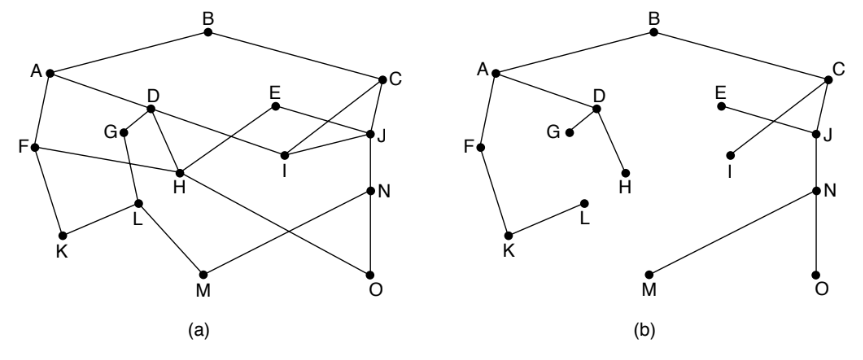
\includegraphics[width=0.7\linewidth]{IN1/IN60.png}
\caption{a. Una red. (b) Un árbol sumidero para el enrutador B.}
\label{fig:optimizacion}
\end{figure}
%----------------------------------------------------------------------------------------
%Microprocesadores
%----------------------------------------------------------------------------------------

%----------------------------------------------------------------------------------------
%Mantenimiento
%----------------------------------------------------------------------------------------

%----------------------------------------------------------------------------------------
\end{document}
%----------------------------------------------------------------------------------------
